\fancyhead[LE,RO]{\color{black}{\thepage}}
\fancyhead[RE,LO]{\subsectionfont\itshape\color{activeColor}Résumé étendu en français}
\fancyfoot[C]{}
\counterwithout{figure}{chapter}
\counterwithout{equation}{chapter}
\setcounter{figure}{0}
\setcounter{equation}{0}
\chapter{Résumé étendu en français}
	\lettrine[lines=4]{\color{activeColor}D}{ans} cette thèse, j'ai étudié deux aspects de la dynamique des impuretés atomiques interagissant avec des nanogouttelettes d'hélium superfluide (He), à savoir la photo-excitation d'atomes d'alcalins sur une nanogouttelette et le dopage de nanogouttelettes contenant des tourbillons quantiques avec des atomes de gaz rares. Pour les investigations théoriques, nous utilisons la théorie de la fonctionnelle de la densité d'hélium (He-DFT), similaire à la DFT électronique mais avec la densité d'hélium à la place de la densité électronique,  et sa version dépendant du temps (He-TDDFT).	

	Le premier aspect de cette étude s'est effectué dans le cadre d'une collaboration avec l'équipe expérimentale de Mudrich et Stienkemeier à Heidelberg.
	Il concerne la photo-excitation du rubidium (Rb). 
	Les atomes d'alcalins constituent une sonde très intéressante des gouttelettes d'He car ils résident dans leur région de surface.
	Dans cette région il a été suggéré qu'un taux de près de 100\% de condensation de Bose-Einstein pouvait être obtenu en raison d'une densité inférieure à celle de l'hélium superfluide  dans le volume.
	
	Le deuxième aspect concerne une investigation purement théorique inspirée par des travaux récents de Gomez et Vilesov \emph{et al}., où les tourbillons quantiques ont été visualisés en dopant des nanoparticules d'He avec des atomes d'argent, puis en les faisant atterrir en douceur (\guillemotleft~soft landing~\guillemotright{}) sur un écran de carbone. 
	Les images au microscope électronique montrent de longs filaments d'agrégats d'atomes d'argent qui s'accumulent le long des noyaux des vortex. La formation de réseaux de tourbillons quantiques à l'intérieur de nanogouttelettes est également mise en évidence en utilisant l'imagerie par diffraction des rayons~X pour visualiser les motifs de Bragg caractéristiques des agrégats de xénon (Xe) piégés à l'intérieur des noyaux des vortex.
	
	Nos simulations impliquant des gouttelettes hébergeant des tourbillons quantiques ouvrent la voie à d'autres investigations sur des gouttelettes hébergeant une série de vortex, impliquant de multiples impuretés.
		
	\section*{Introduction \small{(Chapitre~1)}}
		Jusqu'aux années 1980, la plupart des travaux expérimentaux et théoriques ont été effectués sur des systèmes macroscopiques, c'est-à-dire des systèmes pour lesquels le nombre d'atomes est de l'ordre de grandeur du nombre d'Avogadro $N_A$. 
		Ce n'est qu'au cours des deux dernières décennies que les progrès technologiques ont permis aux expérimentateurs d'obtenir des gouttelettes d'hélium superfluides de taille nanométrique. 
		Dès le début des années 1990, les nanogouttelettes d'hélium superfluides sont devenues un champ d'étude actif, tant sur le plan expérimental que théorique. 
		
		Les nanogouttelettes d'hélium sont considérées comme des systèmes modèles idéaux pour explorer l'hydrodynamique quantique dans des superfluides autonomes et isolés. 
		L'objectif principal a été l'évolution de leurs propriétés en fonction du nombre d'atomes, depuis l'agrégat de petite taille  jusqu'à la limite de la matière condensée. 
		Les agrégats d'hélium sont particulièrement intéressants dans la mesure où les effets quantiques jouent un rôle clé dans la détermination de leurs propriétés. 
		En particulier, étant donné qu'une nanogouttelette d'hélium constitue un ensemble de bosons à environ 0.4~K\citep{Brink1990, Hartmann1995}, des manifestations de comportement collectif (comme la superfluidité) sont attendues. 
		D'autre part, il n'est pas encore clair comment la taille finie de cet ensemble affecte ce comportement collectif non-classique.

		Récemment, Toennies \emph{et al}. ont mesuré le spectre électronique de molécules de glyoxal solvatées dans des nanogouttelettes d'hélium,\citep{Hartmann1996} et l'ont trouvé compatible avec une simulation théorique utilisant la courbe de dispersion de phonons d'He II superfluide macroscopique. 
		Les auteurs eux-mêmes soulignent cependant que pour la taille moyenne des nanogouttelettes dans lesquelles ont été effectuées les expériences, qui était de 5500 atomes d'He, \rf{Hartmann1996}, les effets de taille finie dans la région intérieure devraient être négligeables (voir aussi\rfs{RamaKrishna1990-1,Chin1992}). 
		Il n'est donc pas surprenant qu'ils trouvent des résultats cohérents avec le cas du superfluide macroscopique, en particulier pour une molécule comme le glyoxal qui est solvatée à l'intérieur de la nanogouttelette, et pour laquelle les effets de surface jouent donc un rôle mineur. 
		Par conséquent, l'influence de la taille des clusters d'He sur la superfluidité n'a pas été déterminée de façon concluante jusqu'à présent.

		L'interaction hélium-hélium est déjà faible dans l'hélium liquide macroscopique. 
		Dans les systèmes auto-liés finis tels que les gouttelettes elle est encore plus faible:  l'énergie de liaison par atome est $<$7.17~K. 
		De ce fait, les gouttelettes d'hélium se refroidissent très rapidement par évaporation, qui est très rapide, et atteignent ainsi leur température limite d'environ 0.38~K en quelques microsecondes. 
		Les gouttelettes d'hélium pur sont des systèmes neutres et leurs propriétés comme leur taille, leur énergie de liaison et leur spectre d'excitation ne sont pas faciles à déterminer expérimentalement.
		Ces propriétés sont généralement obtenues par des méthodes indirectes.
	   Cela n'a pas empêché les théoriciens de décrire des gouttelettes dopées $^4$He$_N$ en utilisant une grande variété d'approches en fonction de la taille et du caractère des gouttelettes.
	   Ces méthodes incluent  Monte Carlo quantique (de diffusion, ou variationnel\citep{Gartner2018}, Hypernetted-Chain/Euler-Lagrange\citep{Krotscheck2001}) et beaucoup d'autres.

		Une propriété remarquable des gouttelettes d'hélium, contrairement à l'hélium liquide macroscopique, est leur capacité à capturer n'importe quel type de dopants avec lesquels ils entrent en collision. 
		En fonction de la force de l'interaction dopant-$^4$He et de la tension superficielle de la gouttelette, on peut définir un paramètre sans dimension $\lambda$\citep{Anc95} avec une valeur critique $\lambda_0\!\!\sim$1.9. 
		Au-dessous de $\lambda_0$, les impuretés sont liées à la surface de la gouttelette (c'est le cas des atomes d'alcalins par exemple) qu'elles déforment pour une meilleure interaction.
		 Au-dessus e $\lambda_0$, elles sont solvatées à l'intérieur de la gouttelette. 
		 Les gouttelettes peuvent donc être dopées avec presque toutes sortes d'espèces atomiques ou moléculaires.

		Du point de vue de la gouttelette, cela signifie qu'il est possible d'utiliser les dopants comme des sondes peu perturbantes pour déterminer les propriétés superfluides des gouttelettes d'hélium qui seraient inaccessibles avec d'autres méthodes. 
		Pour deux exemples de ceci, voir\rfs{Gre98,Sin89,RamaKrishna1990-2}, où un dopant est utilisé pour sonder le caractère superfluide de petites gouttelettes d'hélium $^4$He et\rfs{Hartmann1999, Harms1999} pour déterminer leur température limite.
		
		De plus, du point de vue des impuretés, la solvatation en nanogouttes d'hélium permet un vaste spectre d'études expérimentales. 
		Du fait que les gouttelettes d'hélium constituent un environnement liquide superfluide ultra-froid, avec très peu d'interaction avec le dopant, on peut réaliser des études de spectroscopie à haute résolution. 
		De plus, en contrôlant finement le nombre de dopants [29], on peut utiliser des gouttelettes comme matrices pour créer des structures auto-organisées de molécules polaires, ou des agrégats de métaux très froids et étudier leur explosion de Coulomb.

		L'une des propriétés les plus intrigantes des gouttelettes d'hélium superfluides est le fait qu'elles peuvent héberger des vortex quantifiés. 
		En raison de leur température ultra basse, ce sont de véritables liquides quantiques et leur moment cinétique est quantifié. 
		L'existence de tourbillons quantiques a été anticipée car ceux-ci ont été créés et observés dans des condensats de Bose-Einstein (BEC) constitués de gaz dilués. 
		Cependant, la détection de tourbillons quantiques est encore expérimentalement difficile (voir \scn{sec:quant-vort} de cette thèse).

		Parmi les nombreux travaux menés sur les gouttelettes d'hélium au cours des dernières décennies, à la fois expérimentalement et théoriquement, on peut citer les spectres d'absorption de gouttelettes d'hélium dopées par des métaux alcalins, l'étude de gouttelettes dopées mixtes $^3$He--$^4$He, celle des électrons dans de l'hélium liquide, l'étude de la vitesse critique de Landau à l'intérieur de petites $^4$He gouttelettes...
		Pour un aperçu plus complet et plus exhaustif, je renvoie aux articles de revue \rfs{Barranco2006,Ancilotto2017,Mudrich2014}.
	
	\section*{Méthodes utilisées \small{(Chapitre~2)}}
		D'un point de vue théorique, l'hélium superfluide doit être considéré comme un système quantique de grande dimension. 
		Les calculs quantiques Monte Carlo\citep{Kro02} (QMC) et quantique direct\citep{deL06,deL10,Agu13} sont les méthodes les plus précises, mais ils demandent des ressources informatiques qui dépassent rapidement les capacités actuellement disponibles lorsque le nombre d'atomes d'hélium augmente. 
		De plus, QMC ne peut pas décrire l'évolution dynamique de l'hélium superfluide en temps réel.
		 Pour pallier ces limitations, des méthodes semi-empiriques basées sur le formalisme de la DFT ont été introduites: \citep{Str87a,Str87b,Dal95}. 
		 La DFT peut être appliquée à des systèmes beaucoup plus grands que QMC et permet une formulation dépendante du temps. 
		 Elle offre le meilleur compromis entre précision, faisabilité computationnelle, et taille réaliste des systèmes traités par rapport aux tailles des systèmes expérimentaux. 
		 Le principal inconvénient de la DFT est que la fonction énergétique exacte n'est pas connue et doit donc être construite de manière semi-empirique. 
		 De plus, la description de l'interaction dopant-hélium dans les gouttelettes d'hélium dopées est limitée à une approche de champ moyen. 
		 Néanmoins, la DFT est la seule méthode à ce jour capable de reproduire avec succès les résultats d'une vaste gamme d'expériences résolues en temps dans l'hélium superfluide, pour des tailles réalistes par rapport aux conditions expérimentales.

		Le point de départ de la méthode fonctionnelle de densité est le théorème de Hohenberg-Kohn\citep{Hohenberg1964} (HK), qui indique que l'énergie de l'état fondamental $E_v$ d'un système \emph{interagir inhomogène} dans un potentiel statique $v$ peut être écrit comme une fonctionnelle unique de la densité à un corps $\rho$, dénotée $F[\rho]$, une  fonctionnelle universelle ---valable pour \emph{n'importe quel} nombre de particules et \emph{n'importe quel} potentiel externe $v$--- de la densité.
		
		Kohn et Sham ont ensuite reformulé\citep{Kohn1965} la théorie en introduisant un schéma d'ap\-pro\-xi\-ma\-tion pour la fonctionnelle $F[\rho]$  qui est analogue à la méthode de Hartree, mais qui contient également la majeure partie des effets de corrélation inhérents à l'interaction des systèmes à plusieurs corps. 
		L'approximation commence par scinder la fonctionnelle en une énergie cinétique et une partie d'énergie de corrélation. 
		L'énergie cinétique est celle d'un système fictif de particules \emph{sans interaction} de densité $\rho$. 
		La partie de corrélation correspond à un système de particules \emph{en interaction} avec la même densité. 
		Pour la partie cinétique, cela nous permet d'écrire l'énergie cinétique totale comme la somme des énergies cinétiques individuelles des particules sans interaction. 
		La différence entre la véritable énergie cinétique du système en interaction et celle du système fictif est prise en compte dans la partie énergie de corrélation. 
		C'est seulement la somme de ces deux termes qui donne l'énergie d'état fondamental correcte pour un système de particules en interaction.
		
		Parce que la fonction que nous avons utilisée dans ce travail est calibrée pour reproduire le bon comportement de l'hélium liquide à température nulle et sans pression, nous supposons une condensation complète de l'hélium entre Bose-Einstein (BE). 
		Dans ce cas, tous les atomes d'hélium occupent le même état fondamental, pris comme orbitale Kohn-Sham. 
		Les expressions de la fonction d'onde à $N$-corps et de la densité se simplifient alors davantage et permettent de décrire l'ensemble du système en définissant une fonction d'onde efficace qui ne dépend que d'une coordonnée dans un espace cartésien à trois dimensions.
		
		La difficulté consiste à concevoir une fonction telle que les propriétés physiques souhaitées de l'hélium puissent être bien décrites. 
		C'est loin d'être trivial mais plusieurs de ces fonctionnelles de la densité sont disponibles à l'heure actuelle. 
		La fonctionnelle de la densité utilisée dans ce travail est basée sur la fonctionnelle d'\emph{Orsay-Trento} qui est discutée dans la \scn{sec:otdft} de la thèse. 
		Elle utilise une approche non locale à échelle finie et constitue, à ce jour, le modèle le plus précis dans la mesure où ses paramètres ont été ajustés pour reproduire les propriétés globales de l'hélium liquide à température nulle.
		
		Dans le cas de densités de liquide hautement inhomogènes, par ex.\ en présence d'impuretés atomiques avec une interaction He-X très forte, la fonctionnelle OT devient numériquement instable. 
		Pour résoudre ce problème, un terme de pénalité énergétique  est ajouté.
		 L'inclusion de ce terme dans la fonctionnelle OT empêche l'accumulation excessive de densité. 
		 La suppression des termes non locaux de la fonction OT d'origine et l'ajout de ce terme de pénalité donnent une fonctionnelle de densité modifiée qui est appelée fonctionnelle du solide \emph{(Solid Functional)}. 
		 Voir \scn{sec:solid} pour plus de détails et pour les valeurs de ses paramètres.
		
		Pour décrire l'évolution temporelle du système, le théorème de Runge-Gross étend la DFT à sa version dépendante du temps TDDFT\citep{Run84}. 
		La variation fonctionnelle de l'action associée (voir \eq{eq:action} pour un exemple) conduit à une équation d'Euler-Lagrange (EL) dépendante du temps. 
		En considérant seulement les états stationnaires du Hamiltonien, on obtient une équation EL indépendante du temps qui, lors de la résolution, donne l'énergie de l'état fondamental du système.
		
		Pour plus de détails sur la façon dont les calculs statiques et dynamiques sont résolus pour les différentes impuretés dans des potentiels d'interactions isotropes et anisotropes, veuillez vous reporter aux Sections~2.3 et 2.4.
		
	\section*{Dynamique d'état excité des nanogouttelettes dopées aux alcalis \small{(Chapitre~3)}}
		Dans un article de 1996\citep{Griffin1996}, Griffin et Stringari ont fait valoir que près de 100\% de condensation de Bose-Einstein pouvait être obtenue dans la région superficielle à faible densité d'He superfluide à $T=0$, contre seulement 10\% dans le volume du liquide. 
		Il est donc évident qu'une sonde à perturbation minimale capable d'étudier la surface d'un cluster He est très souhaitable.
		
		Il a été proposé d'un point de vue théorique\citep{Dalfovo1994} que les atomes d'alcalins résident sur la surface de la nanogoutte. 
		Des preuves expérimentales ont été trouvées \citep{Stienkemeier1995-1,Stienkemeier1995-2,Ancilotto1995-1} plus tard quand il a été observé que le spectre de fluorescence induite par laser (LIF) du sodium était déplacé par rapport à celui du sodium dans la phase gazeuse en raison de la présence de l'environnement d'hélium,  mais seulement d'environ la moitié par rapport à celui du même alcalin à l'intérieur de l'hélium liquide.
		
		Les atomes d'alcalins sont donc un choix très naturel pour ce type d'études. 
		Par exemple, avec un paramètre de solvatation (voir \scn{sec:helium-droplets})  $\lambda$ de 0.729\citep{Anc95}, Rb reste lié à la surface de la gouttelette. 
		De plus, les atomes d'alcalin ont un spectre d'absorption simple et bien connu. 
		Par ailleurs, leur structure électronique simple à un électron de valence permet une modélisation théorique détaillée. 
		Ces atomes n'introduisent que des perturbations faibles (les énergies d'interaction alcalin-hélium sont de l'ordre de 1~cm$^{-1}$\citep{Pat91}). 
		Enfin, des calculs théoriques\citep{Ancilotto1995-2,Kanorsky1994} et des spectres expérimentaux\citep{Tabbert1995,Takahashi1993,Beijersbergen1993} d'atomes d'alcalins à l'intérieur de l'hélium liquide sont disponibles à titre de comparaison.
		
		Les transitions $n\mathrm{p}\,^2\mathrm{P}\!\leftarrow\!n\mathrm{s}\,^2\mathrm{S}$  des atomes d'alcalins ont suscité beaucoup d'intérêt d'un point de vue expérimental aussi bien que théorique. 
		La spectroscopie des états excités supérieurs a été largement explorée\citep{Log11b,Log11a,Lackner2012,Lackner2013,The11,Fec12,Pif10,Lac11,Theisen2011,Lac13}.
		 Les spectres obtenus peuvent être reproduits avec succès par un modèle pseudo-diatomique dans lequel la nanogouttelette est représentée par un pseudo-atome.
		 Pour les états excités supérieurs, ce modèle échoue progressivement en raison des limitations de son domaine de validité\citep{Sti96,Bunermann2007}. 
		 Alors que l'effet de l'environnement d'une nanogoutte d'hélium sur le spectre des états excités d'un alcalin en sa surface est maintenant assez bien compris, la dynamique induite par l'excitation d'un de ces états est peu explorée.
		
		Dans cette partie de la thèse, les résultats de la dynamique en temps réel d'un seul atome de rubidium (Rb) électroniquement excité résidant initialement dans une cuvette en surface d'une nano-gouttelette d'hélium sont présentés. 
		L'atome est excité depuis son état fondamental 5s$\,^2\Sigma_{1/2}$ vers les états 5p$\,^2\{\Sigma,\Pi\}$ et 6p$\,^2\{\Sigma,\Pi\}$  (voir \scn{sec:dim-model} pour une explication des étiquettes d'état électroniques utilisées). 
		Habituellement, cette excitation provoque la désorption soit de l'atome nu, soit  d'un complexe de l'alcalin avec un ou plusieurs atomes d'hélium, appelé un \guillemotleft~exciplexe~\guillemotright.	
	
	\section*{Imager la dynamique des états excités \small{(Chapitre~4)}}
		\begin{figure}
			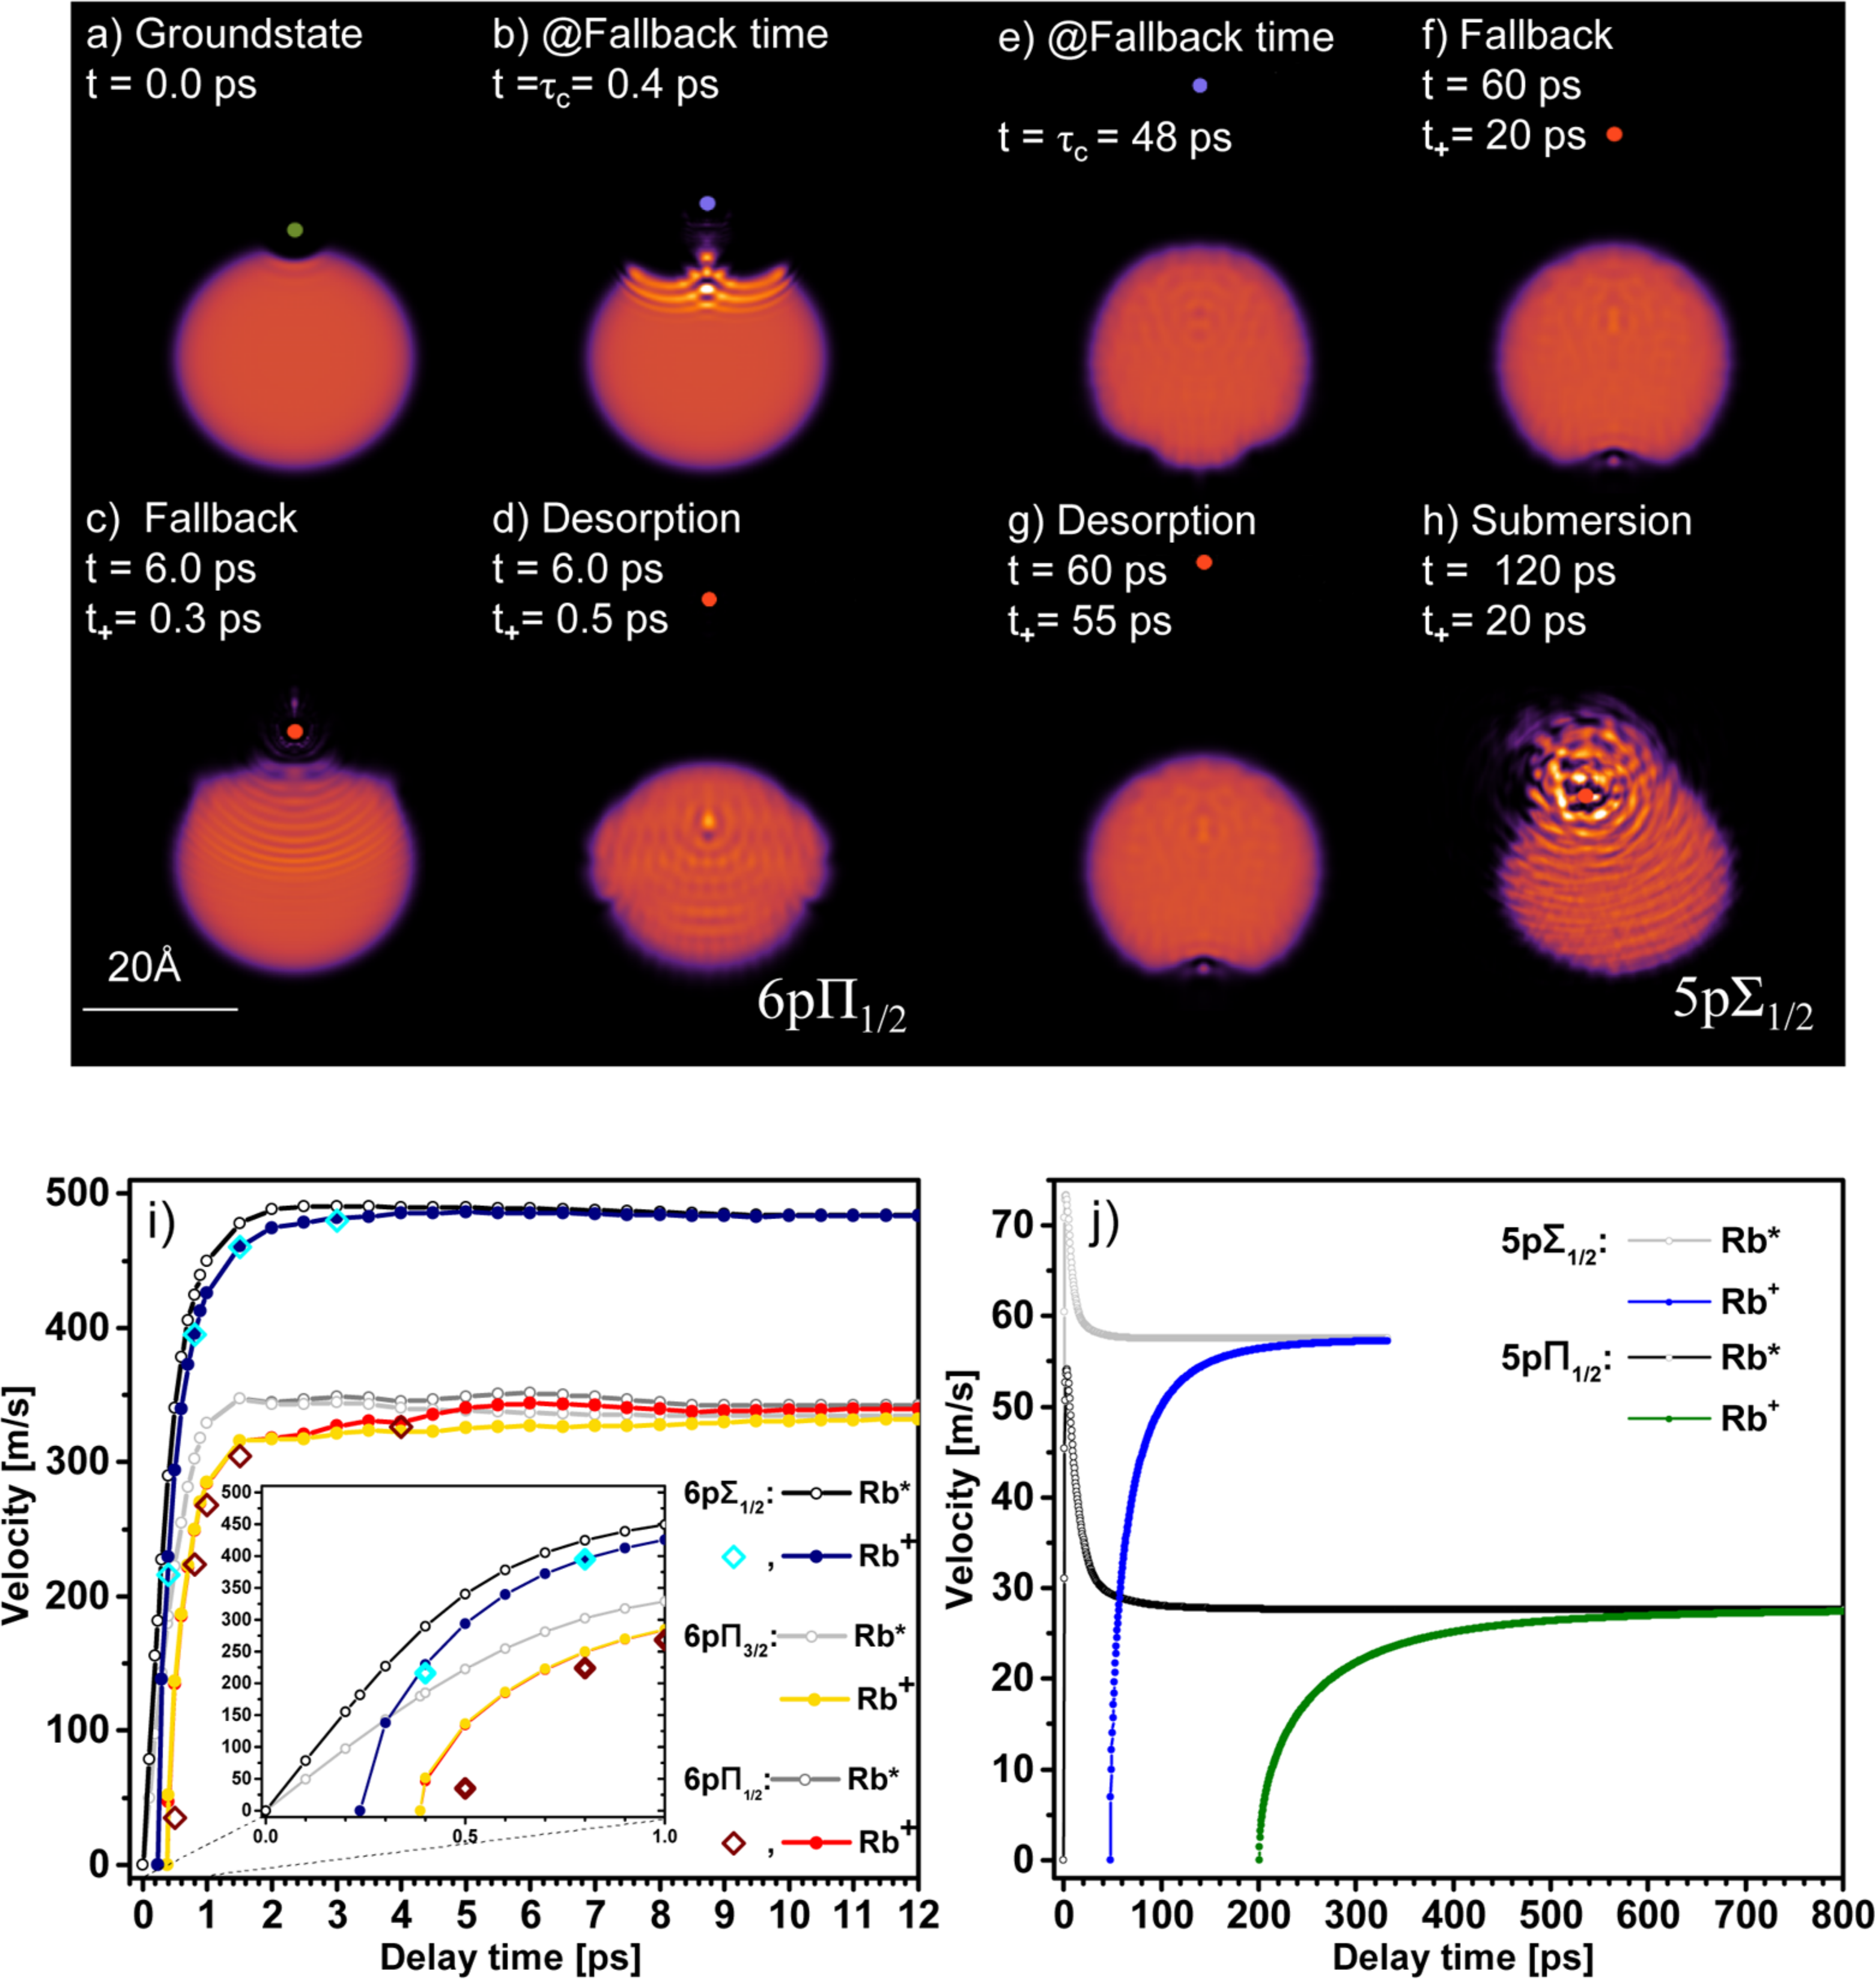
\includegraphics[width=\linewidth]{fallback-time}\label{fig:fallback-time}
			\caption{Densités 2D (a−d,e−h) et vitesses basées sur TDDFT (i,j) pour un atome de Rb attaché à une goutellette He$_{1000}$ et excité depuis l'équilibre (a) vers des états 6p (colonne de gauche) et 5p (colonne de droite). 
			Les densités sont représentées pour différents temps total de propagation $t$ et différents instants d'ionisation $t_+$ : (b,e) Rb neutre à  $t=\tau_c$ (\guillemotleft~fall-back time~\guillemotright{}, temps critique de retour); (c,f) ionisation à $t_+<\tau_c$, l'ion Rb$^+$ retombe sur la nanogouttelette; (d,g) $t_+>\tau_c$, désorption de Rb$^+$ ; (h) solvatation de Rb$^+$ ; (i,j) évolution des vitesses Rb* avec le temps $t$ (symboles gris vides), et vitesses finales de Rb$^+$ (symboles pleins) en fonction de $t_+$. (Voir Chapitre~\ref{ch:exc-state-dyn} de la thèse.)}
		\end{figure}		
		Le  Chapitre~4 correspond à une étude combinée expérimentale et théorique centrée sur l'imagerie et la caractérisation de la dynamique induite par les excitations 5p$\leftarrow$5s et 6p$\leftarrow$5s du rubidium hébergé par une nanogouttelette d'hélium. 
		L'expérience a utilisé des techniques pompe-sonde à l'échelle femtoseconde, avec un premier laser excitant le Rb sur la surface des gouttelettes au temps $t_{exc}$ et un second laser l'ionisant pour la détection par imagerie des vecteurs vitesse (VMI) au temps $t_{ion}$. 
		Les résultats ont permis de caractériser un délai critique $\tau_c$, appelé \guillemotleft~fall-back time~\guillemotright (temps de retour), entre deux processus opposés. 
		Si $t_{ion}-t_{exc}\leq\tau_c$, l'atome Rb sortant est encore assez proche de la gouttelette pour que l'énergie d'attraction dans l'état ionique atteint par le laser sonde soit supérieure à son énergie cinétique. 
		Par conséquent, le Rb$^+$ fait demi-tour et il finit solvaté. 
		A l'opposé, pour $t_{ion}-t_{exc}\geq\tau_c$, l'ionisation se produit trop tard pour que Rb$^+$ ressente une attraction appréciable de la part de la gouttelette, et il avait déjà trop d'énergie cinétique, il s'échappe.
		
		L'étude théorique a porté sur la compréhension de la dynamique de désorption et sur la détermination des temps de retour, pour comparer avec l'expérience. 
		Elle a fait usage de l'He-TDDFT présentée dans \scn{sec:td-dft}, à la fois dans les états excités et les états ionisés. 
		Les résultats sont présentés dans l'article incorporé à la suite dans ce chapitre, article qui a été publié dans le Journal of Physical Chemistry Letters\citep{Vangerow2017}.
		
		Dans nos simulations, nous trouvons que les états excités 5p et 6p désorbent à des échelles de temps très différentes, séparées par deux ordres de grandeur ($\sim$100~ps et $\sim$1~ps pour respectivement 5p et 6p). 
		Ceci est en bon accord avec les résultats expérimentaux, et permet de conclure à un processus impulsif de désorption par excitation dans le cas de l'excitation 6p, alors que le mécanisme de désorption pour l'excitation 5p est plus complexe.

	\section*{Dynamique de désorption des exciplexes RbHe \small{(Chapitre~5)}}
		\begin{figure}
			\centering
			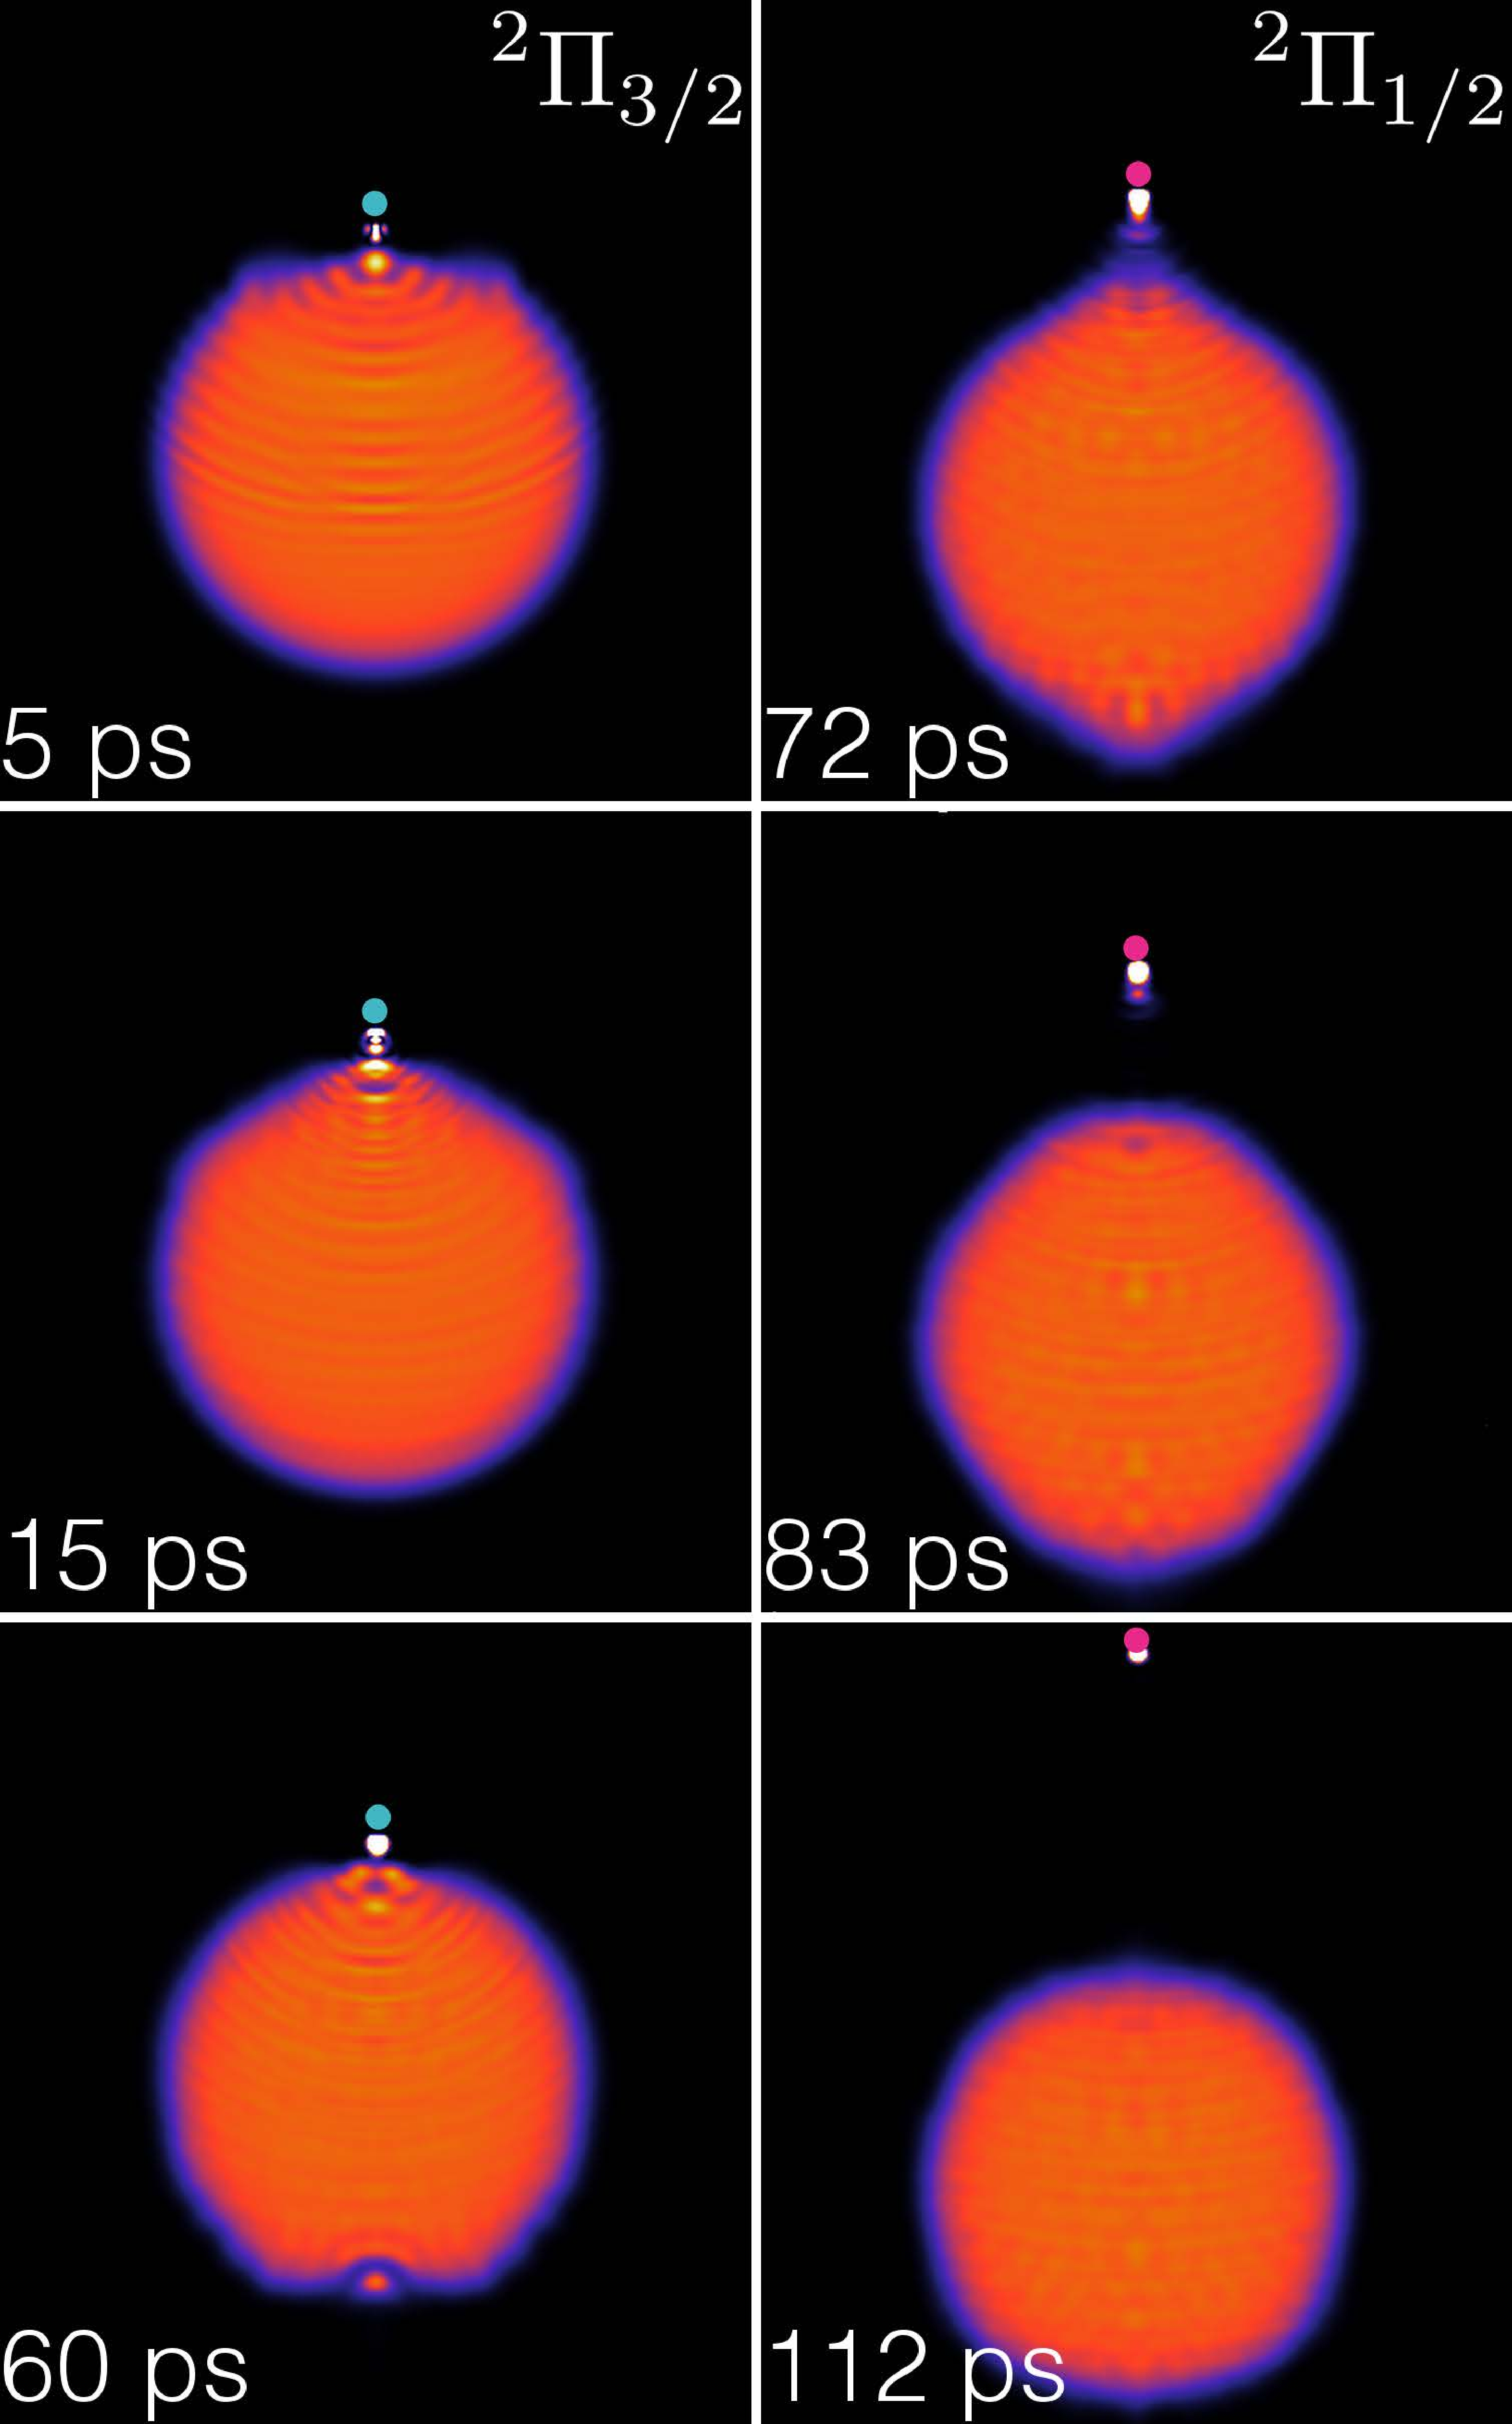
\includegraphics[width=0.9\linewidth]{fig5-pccp}\caption{Instantanés de la densité de l'hélium au cours de l'évolution du complexe RbHe$_{1000}$ excité pour $\eta$=15\%,~$\Delta t$=60~ps. Le point vert représente l'atome Rb, excité à l'état 5p$\Pi_{3/2}$ ; le point magenta est l'atome Rb après une relaxation soudaine à l'état 5p$\Pi_{1/2}$. (Voir Chapitre~\ref{ch:rbhe-exciplexe} de la thèse.)}
			\label{fig:snapshots}
		\end{figure}	
		Les résultats du Chapitre~4 montre un bon accord théorie-expérience pour les états 6p et $\,^2\Sigma_{1/2}$  et $\,^2\Pi_{1/2}$ de l'excitation 5p.
		Par contre, dans nos simulations, l'excitation à l'état 5p$\,^2\Pi_{3/2}$ aboutit à un exciplexe de RbHe lié à la surface, contrairement au cas expérimental où un exciplexe RbHe est bien formé, mais il désorbe de la surface des gouttelettes. 
		Comment résoudre cette apparent désaccord?
		C'est la question qui a conduit à ce travail.
	    Nous avons montré qu'en introduisant la relaxation de spin $^2\Pi_{1/2}\!\leftarrow\!^2\Pi_{3/2}$ dans les simulations, l'exciplexe RbHe est capable de désorber à partir de la surface de la gouttelette, ce qui résout cette contradiction.
		
		Lors de la photo-excitation de Rb à l'état 5p$\,^2\Pi_{3/2}$, un atome d'He peut s'y  attacher, formant ainsi un exciplexe HeRb.
		Ce processus ne peut pas se produire si Rb est excité à l'état 5p$\,^2\Pi_{1/2}$ à cause de l'existence d'une barrière (voir \fig{fig:potentials}) qui empêche la formation d'exciplexe.
		
		Dans la phase gazeuse, un exciplexe HeRb~5p$\,^2\Pi_{1/2}$ peut être formé s'il y a assez d'énergie cinétique pour que Rb* surmonte la barrière de potentiel.
		Alternativement, la collision de l'exciplexe HeRb~5p$\,^2\Pi_{3/2}$ avec un autre atome ou complexe pourrait faire relaxer l'atome Rb* de l'état 5p$\,^2\Pi_{3/2}$ vers l'état 5p$\,^2\Pi_{1/2}$, surmontant alors la barrière car les puits de potentiel pour les deux états sont à des distances Rb-He similaires. 
		En surface des nanogouttelettes à la température de 0.4~K, aucun de ces mécanismes n'est disponible pour expliquer la formation des exciplexes HeRb~5p$\,^2\Pi_{1/2}$ et leur éjection potentielle.
		
		Cependant,  la désexcitation non radiative de l'atome Rb*  depuis l'état 5p$\,^2\Pi_{3/2}$ vers l'état 5p$\,^2\Pi_{1/2}$ fournit assez d'énergie pour que l'atome ou l'exciplexe puisse être éjecté. 
		Notez dans la \fig{fig:potentials} que le minimum du potentiel 5p$\,^2\Pi_{3/2}$ est à 12683~cm$^{-1}$, et celui du 5p$\,^2\Pi_{1/2}$ potentiel est à 12518~cm$^{-1}$; la valeur de ce potentiel à la barrière est de 12611~cm$^{-1}$. 
		Ainsi, une désexcitation non radiative de l'atome Rb* peut ajouter à son énergie cinétique d'origine jusqu'à 165~cm$^{-1}$. 
		Il est à noter qu'il sera éjecté dans l'état 5p$\,^2\Pi_{1/2}$, et non dans le 5p$\,^2\Pi_{3/2}$ où il était précédemment photo-excité, mais les mesures expérimentales ne permettaient pas de déterminer l'état électronique final de l'atome ou de l'exciplexe.
		
		Les simulations ont consisté à induire de façon soudaine la relaxation vers l'état 5p$\,^2\Pi_{1/2}$ (après une phase de stabilisation dans l'état 5p$\,^2\Pi_{3/2}$), et à attribuer au Rb$^*$ une proportion $\eta$ des 165~cm$^{-1}$ d'énergie disponible.
		Nous avons conclu qu'une proportion $\eta=15$~\% permettait de reproduire l'expulsion, et d'obtenir un bon accord avec les résultats expérimentaux.
		Cette étude a fait l'objet d'une publication.
%		Cette publication contient une extension de notre recherche expérimentale et théorique combinée présentée dans la section précédente. Nous nous intéressons ici à la formation de molécules de RbHe-exciplex libres à partir de nanoparticules d'He dopées au Rb et excitées par laser grâce au mécanisme de relaxation de spin électronique.

	\section*{Nanogouttelettes de potassium dopées \small{(Chapitre~6)}}
		Sous la supervision de Nadine Halberstadt et moi-même, un projet de recherche M2  ---\emph{M2 Physique Fondamentale}--- intitulé \emph{\textbf{\guillemotleft~Dynamique d'une nanogouttelette d'hélium superfluide dopée avec un seul atome de potassium~\guillemotright}} a été mené par Maxime Martinez.
		
		Ce projet étudiait le comportement statique et dynamique d'un atome de potassium (K) excité de la configuration d'équilibre K-$^4$He$_{1000}$ aux états K*(4p)-$^4$He$_{1000}$ et K*(5s)-$^4$He$_{1000}$. 
		Le choix du potassium a été motivé par un désaccord dans les études expérimentales résolues en temps\citep{Schulz2001,Reho2000-1,Reho2000-2} sur les constantes de temps pour la désorption. 
		De plus, la masse de potassium se situe entre celles des alcalins plus lourds comme le rubidium et le césium, et les plus légers, comme le lithium et le sodium. 
		Par conséquent, le potassium présente un cas intéressant, étant à la limite entre le régime classique pour les alcalins lourds et un régime quantique pour les plus légers. 
		Les deux approches pour la description du potassium, classique et quantique, sont testées pour la description des propriétés d'équilibre et de l'excitation 5s $\leftarrow$ 4s. 
		Ce travail n'est pas inclus dans cette thèse mais peut être trouvé à la \rf{Martinez2017}.
		
		On conclut que les effets quantiques de K existent mais ne sont pas essentiels à la compréhension et à la description de la dynamique. 
		Donc l'excitation K*(4p)-$^4$He$_{1000}$ est étudiée avec une description classique de K.

	\section*{Tourbillons quantifiés en gouttelettes \small(Chapitre~7)}
		Le deuxième aspect de la dynamique d'impuretés atomiques en interaction avec des nanogouttelettes d'hélium étudié dans cette thèse concerne une investigation purement théorique inspirée par des travaux récents de Gomez et Vilesov \emph{et al}.
		Dans ces expériences, les tourbillons quantifiés ont été visualisés en dopant des nanoparticules d'He avec des atomes d'argent, puis en les faisant atterrir en douceur (\guillemotleft~soft landing~\guillemotright{}) sur un écran de carbone. 
		Les images au microscope électronique montrent de longs filaments d'agrégats d'atomes d'argent qui s'accumulent le long des noyaux des vortex. 
		La formation de réseaux de tourbillons quantiques à l'intérieur de nanogouttelettes est également mise en évidence en utilisant l'imagerie par diffraction des rayons~X pour visualiser les motifs de Bragg caractéristiques des agrégats de xénon (Xe) piégés à l'intérieur des noyaux de vortex.
		
		L'une des signatures les plus claires de la nature quantique d'une substance - et en fait de la superfluidité - est l'apparition de vortex quantiques. 
		Contrairement à un fluide normal, qui tourne comme un corps solide lorsque son récipient se déplace à une faible vitesse angulaire, un superfluide reste au repos. 
		Cependant, au-dessus d'une certaine vitesse angulaire critique, l'état thermodynamiquement stable d'un superfluide comprend un ou plusieurs vortex quantiques. 
		Un tel vortex peut être caractérisé par une fonction d'onde macroscopique et une circulation de vitesse quantifiée en unités de $\kappa=\frac{h}{m}$, où $h$ est la constante de Planck et $m$ est la masse d'un atome $^4$He\citep{Don91,Pit03}. 
		Récemment, l'étude de la vorticité a été étendue à des systèmes finis tels que les condensats de Bose-Einstein (BEC) confinés dans des pièges\citep{Pit03,Fetter2009}. 
		Le transfert d'énergie et de moment cinétique dans les systèmes finis entre les tourbillons quantiques et les excitations de surface est particulièrement intéressant car il définit la dynamique de nucléation, la forme et la stabilité des vortex impliqués\citep{Pit03,Fetter2009}. 
		En comparaison avec les BEC confinés, les gouttelettes $^4$He sont autonomes et présentent un cas de superfluide à interaction forte. 
		De plus, le diamètre d'un noyau de vortex est d'environ 0,2 nm dans le superfluide $^4$He\citep{Don91}, ce qui est petit par rapport à la taille des gouttelettes, et suggère une tridimensionnalité des vortex dans les gouttelettes. 
		Les tourbillons quantiques dans des  gouttelettes d'$^4$He a donc attiré un intérêt considérable\citep{Clo98,Lehmann2003,Bar06,Sti06}.
		
		Dans les expériences de Gomez \emph{et al}.\ citées plus haut,\citep{Gom12}  les tourbillons à l'intérieur des gouttelettes superfluides $^4$He, produites par l'expansion d'hélium liquide, ont été détectés en introduisant des atomes d'argent qui se groupaient le long des lignes de vortex dans les gouttelettes. 
		Les gouttelettes d'hélium nécessaires à ce type d'expériences doivent être plus grandes que celles pour la spectroscopie atomique simple et les études de dynamique car elles doivent être suffisamment grandes pour pouvoir héberger une série de vortex dopés avec de nombreux agrégats d'Ag. 
		Un schéma du principe expérimental est montré dans la \fig{fig:vortex-machine}. 
		Les gouttelettes d'hélium sont produites par détente d'hélium, à 20 bars et à une température $T_0$=5.4-7~K, dans le vide à travers une buse. 
		Les gouttelettes refroidissent rapidement par évaporation et atteignent une température de 0.37~K\citep{Hartmann1995}, ce qui est bien en dessous de la température de transition superfluide $T_\lambda=2.17\unit{K}$\citep{Don91,Pit03}. 
		Plus loin en aval, les gouttelettes capturent 10 atomes de dopant en passant au travers d'un four\citep{Log11d}. 
		Les gouttelettes sont ensuite déposées sur un substrat de film de carbone mince à température ambiante\citep{Log11d}. 
		Lors de l'impact, les gouttelettes s'évaporent, laissant sur la surface des traces d'Ag, qui sont ensuite visualisées par un microscope électronique à transmission (TEM). 
		La prévalence de dépôts allongés en forme de piste (voir \fig{fig:silver-filament}) montre que les tourbillons sont présents dans des gouttelettes de plus de 300~nm et que leur durée de vie dépasse quelques millisecondes.
		
		Deux ans plus tard Gomez \emph{et al}. ont publié un article\citep{Gom14} sur la formation de réseaux de vortex quantiques à l'intérieur des gouttelettes d'hélium. 
		Ils ont utilisé l'imagerie par diffraction de rayons~X femtoseconde à une seule prise pour étudier la rotation de gouttelettes d'hélium-4 superfluides seules, isolées, contenant environ 10$^8$-10$^{11}$~atomes. 
		La formation de réseaux de vortex quantique à l'intérieur des gouttelettes a été confirmée en observant les spectres de Bragg caractéristiques des agrégats de xénons piégés dans les noyaux des vortex (voir la \fig{fig:vortex-array}).
	
	\section*{Collisions frontales \small(Chapitre~8)}
		\begin{figure}
			\centerline{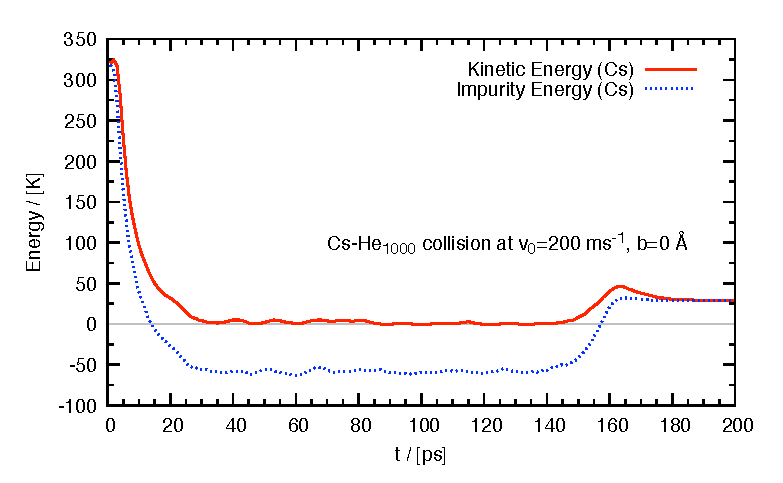
\includegraphics[width=\linewidth]{fig3-Cs-He}} 
			\centerline{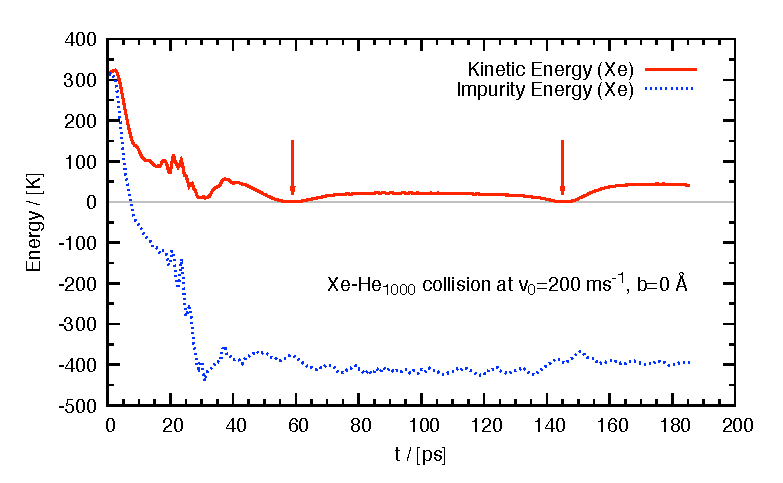
\includegraphics[width=\linewidth]{fig3-Xe-He}}
			\caption{\label{fig3-headon}Figure supérieure : Énergie cinétique et totale (cinétique et potentielle) en fonction du temps d'un atome de Cs, collision frontale contre une gouttelette de $^4$He$_{1000}$ à $v_0$=200~m/s. Figure inférieur : même que le figure supérieur pour un atome de Xe. Les flèches verticales indiquent les deux premiers points de virage à 59 et 145~ps, dont les densités d'hélium correspondantes sont indiquées dans la colonne de droite de la \fig{fig2-headon}.  (Voir Chapitre~\ref{ch:head-on-xece} de la thèse.)}
		\end{figure}	
		Motivés par des expériences récentes utilisant des atomes Xe pour visualiser des réseaux de vortex dans de très grandes gouttelettes d'hélium\citep{Gom14,Jon16}, j'ai abordé dans un premier temps la description de la capture d'atomes de Xe par des gouttelettes d'hélium lors de collisions d'atomes de xénon contre une gouttelette $^4$He$_{1000}$. 
		Cette première étape prépare une étude future sur la capture dynamique des atomes de Xe par des gouttelettes hébergeant plusieurs lignes de vortex, combinant la simulation DFT des réseaux de vortex comme dans les \rfs{Anc14,Anc15} pour les nanocylindres et nanogouttelettes d'hélium et la collision avec les atomes de Xe de ce travail. 
		Dans la mesure du possible, les résultats pour Xe, qui est  héliophile, sont mis en contraste avec les résultats pour Cs, un atome héliophobe de masse similaire.
		
		Les simulations sont effectuées pour une gouttelette de $N=1000$ atomes d'hélium. 
		Sa structure d'état fondamental est obtenue en utilisant la He-DFT, qui donne un rayon d'environ 22.2~\AA. 
		Ensuite, la dynamique est initiée en plaçant l'atome Xe à 32~\AA{}  du centre de masse (COM) de la gouttelette avec un paramètre d'impact égal à zéro (collision frontale). 
		Différentes  vitesses initiales $v_0$ sont testées pour le xénon,  de 200 à 600~m/s dans le système de référence de la gouttelette, ce qui correspond à des énergies cinétiques comprises entre 315.8~K et 2842~K. 
		Ces énergies peuvent être comparées à l'énergie de solvatation d'un atome de Xe au centre d'une gouttelette $^4$He$_{1000}$, $S_{{\rm Xe}}=E({\rm Xe}@^4{\rm He}_{1000})-E(^4{\rm He}_{1000})=-$316.3~K. 
		Par comparaison, l'énergie de solvatation de Cs est de -5.2~K et sa position d'équilibre est dans une cuvette à la surface extérieure des gouttelettes, à environ 26.6~\AA{} de son centre.
		
		Dans les expériences\citep{Gom14,Jon16}, les atomes Xe sont à des vitesses thermiques  ($v_0\!\!\sim$240~m/s), et la vitesse moyenne des gouttelettes est d'environ 170~m/s\citep{Gom11}.
		
		Les résutats montrent que les collisions frontales de nanogouttelettes d'hélium avec du xénon, un atome héliophile, impliquent un échange d'énergie cinétique du même ordre de grandeur que le césium, un atome héliophobe de masse similaire. 
		Dans les deux cas, cette énergie est largement dissipée par la production d'ondes énergétiques dans la gouttelette, ou bien elle est emportée par des atomes d'hélium rapidement émis. 
		La différence entre les deux atomes (Xe ou Cs) est due à la nature différente de leur interaction avec l'hélium. 
		Une accumulation de densité est observée autour du xénon héliophile lors de la dynamique, alors qu'une bulle est créée autour du césium héliophobe. 
		Il faut donc une vitesse initiale beaucoup plus grande pour le xénon pour qu'il traverse la gouttelette et s'échappe que pour le césium, comme on pouvait s'y attendre.
	
	\section*{Capture par He gouttelettes \small(Chapitre~9)}
		Récemment, une technique a été introduite pour déterminer la taille des grosses gouttelettes d'He ($N>10^5$). 
		Elle est basée sur l'atténuation d'un faisceau continu de gouttelettes par des collisions avec des atomes d'Ar à température ambiante\citep{Gom11}. 
		La chambre de dopage de l'appareil à faisceau de gouttelettes est remplie d'argon gazeux et les gouttelettes d'hélium subissent de multiples collisions isotropes avec les atomes Ar sur leur chemin vers la chambre de détection.
		
		De grosses gouttelettes d'hélium peuvent également être dopées de cette manière. 
		Cette méthode, utilisant des atomes Xe, a été instrumentale pour la détection et l'imagerie des réseaux de vortex quantifiés dans les gouttelettes d'hélium\citep{Gom14,Jones2016}. 
		Des atomes Xe ont été utilisés dans ces expériences en raison de leur grande sensibilité à l'imagerie par diffraction cohérente aux rayons~X utilisée pour les détecter dans les gouttelettes d'hélium. 
		Des expériences avec de grandes gouttelettes d'hélium superfluides sont passées en revue dans une publication récente\citep{Tan17}.
		
		L'interaction impureté-gouttelette en présence de vortex est également pertinente en tant que première étape d'un processus plus complexe conduisant à la formation de nanofils, voir par exemple\rfs{Lebedev2011,Gom12,Lat14,Tha14}. 
		Des filaments longs constitués de particules d'hydrogène solides de taille micrométrique piégées sur des noyaux vortex quantifiés ont été utilisés pour imager directement la reconnection  entre les vortex quantifiés dans l'hélium superfluide\citep{Bewley2008}.
		
		Dans cette thèse nous présentons les résultats obtenus par la TDDFT pour la collision et la capture des atomes Xe et Ar par une gouttelette $^4$He$_{1000}$ à différentes énergies cinétiques et paramètres d'impact. 
		Une attention particulière est accordée à l'interaction dépendante du temps des atomes de Xe et d'Ar avec des nanogouttelettes d'hélium contenant des lignes de vortex, et à l'effet de réseaux de tourbillons dopés  dans de grosses gouttelettes d'hélium.
		
		En raison du coût de calcul élevé des simulations TDDFT pour ces systèmes, j'ai abordé seulement quelques facettes du processus de capture qui sont pertinentes pour les comparaisons avec les expériences plutôt que d'effectuer une étude systématique du processus. 
		En particulier:
		\begin{itemize}
			\item J'ai étudié la capture d'atomes de Xe par une nanogoutte de $^4$He, à la fois pour des collisions frontales et pour différents paramètres d'impact, avec des vitesses de valeurs thermiques allant jusqu'à plusieurs centaines de m / s. 
			Les résultats des collisions périphériques avec différentes valeurs du paramètre d'impact sont utilisés pour estimer la section efficace pour la capture du Xe.
			\item J'ai étudié comment un atome de Xe interagit dynamiquement avec une gouttelette hébergeant une ligne de vortex, avec différentes conditions initiales correspondant à différents régimes de vitesse de l'impureté lorsqu'elle entre en collision avec le noyau du vortex:
			\begin{enumerate}
				\item[i)] un atome Xe initialement au repos sur la surface des gouttelettes et s'enfonçant sous l'effet des forces de solvatation;
				\item[ii)] une collision frontale d'un atome Xe ou Ar en mouvement contre la nanogouttelette de $^4$He.
			\end{enumerate}
			\item J'ai étudié l'état stationnaire d'une grosse gouttelette de $^4$He$_{15000}$ contenant un anneau de six lignes de vortex dopées avec des atomes d'Ar remplissant complètement les six noyaux des vortex. 
			C'est le système le plus simple qui imite ceux décrits expérimentalement dans la\rf{Gom14}, où des réseaux de vortex dopés incorporés dans des microgouttes de $^4$He en rotation ont été imagés.
		\end{itemize}

		\subsection*{Capture par des gouttelettes sans vortex}
			J'ai simulé des collisions frontales d'un atome Xe avec une gouttelette $^4$He$_{1000}$ à des vitesses relatives $v_0$ allant de 200 à 600~m/s. 
			La \fig{fig1-capture} montre les diagrammes en deux dimensions de la densité d'hélium pour la valeur la plus élevée, $v_0\!=$600~m/s. 
			Cette vitesse est bien au-dessus de la plage typiquement rencontrée dans les expériences\citep{Gom11,Gom14,Jones2016}. 
			Malgré l'apparition d'une densité d'hélium déconnectée dans le cadre $t$=87~ps, la simulation montre que l'atome Xe fait finalement demi-tour et est à nouveau capturé à l'intérieur de la gouttelette même à cette vitesse d'impact relativement élevée. 
			Notez que l'impureté Xe, même lorsqu'elle émerge temporairement de la gouttelette, apparaît recouverte de quelques atomes de $^4$He, voir la configuration à 87~ps.

		\subsection*{Tourbillons de ligne}
			Pour déterminer la structure d'une gouttelette hébergeant un tourbillon linéaire quantique, la propagation en temps imaginaire est lancée à partir d'une densité d'hélium dans laquelle le tourbillon est \guillemotleft~imprimé~\guillemotright. 
			A cet effet, une ligne de vortex le long de $z$ peut être décrite par la fonction d'onde effective 
			\begin{equation}
				\Psi_0(\mathbf{r}) = \rho_0^{1/2}(r)\,\mathrm{e}^{i\,{\mathcal S}(\mathbf{r})} = \rho_0^{1/2}(\mathbf{r}) \, \frac{(x + i y)}{\sqrt{x^2 + y^2}} \label{eq11-sum}
			\end{equation}
			où $\rho_0(\mathbf{r})$ est la densité de la gouttelette pure ou dopée par une impureté dopée mais sans vortex. 
			Les lignes de vortex le long d'autres directions passant par un point choisi peuvent également être imprimées de cette façon\citep{Pi07}.

			Dans le cas représenté par l'\eq{eq11-sum}, si l'impureté est dans le vortex le long d'un axe de symétrie du complexe impureté-gouttelette, la fonction d'onde effective $\Psi_0({\mathbf r})$ ---avant et après relaxation--- est un vecteur propre de l'opérateur de moment angulaire $\hat{L}_z=-i\,\hbar\partial/\partial\theta$.
			Le moment angulaire de la gouttelette est alors
			\begin{equation}
				\langle \hat{L}_z \rangle = \langle \Psi_0(\mathbf{r}) | \hat{L}_z | \Psi_0(\mathbf{r}) \rangle = N \; \hbar
				\label{eq12-sum}
			\end{equation}

	\subsection*{Dynamique de capture par les tourbillons quantiques}
		\begin{figure}
			\centering
			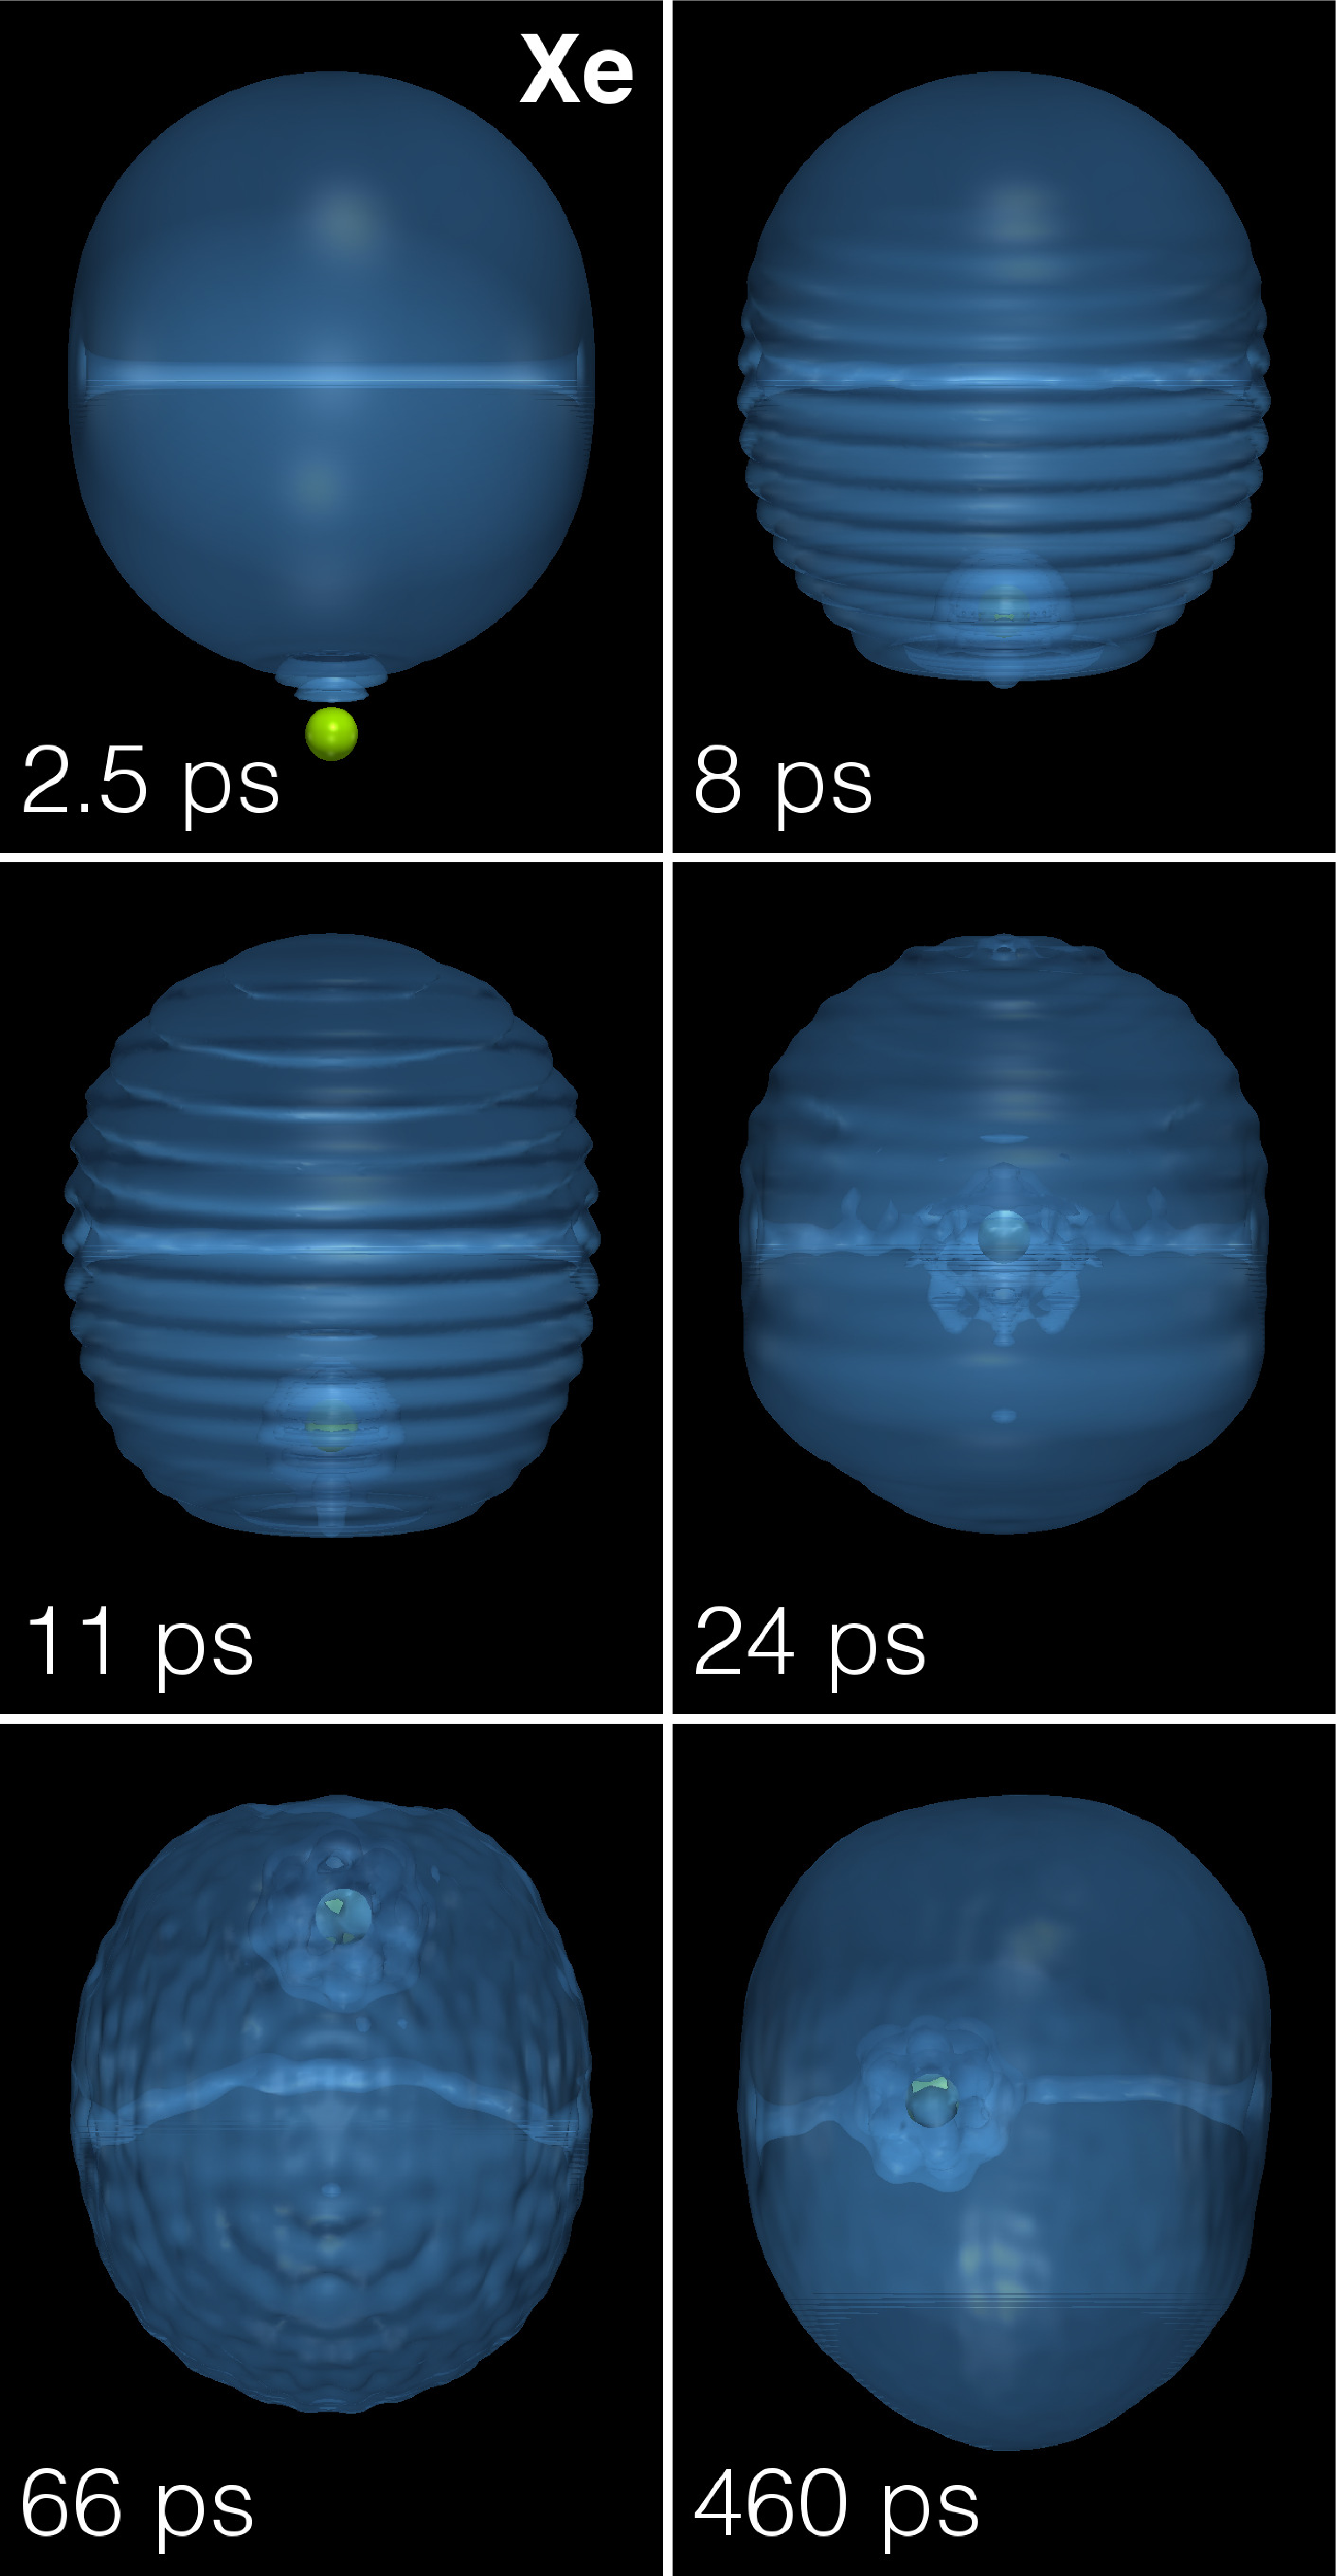
\includegraphics[width=0.75\linewidth]{fig10}
			\caption{\label{fig10-capture}
			Evolution dynamique d'un atome de Xe (point vert) en collision avec une gouttelette de $^4$He$_{1000}$ hébergeant une ligne de vortex à $v_0$=200~m/s. 
			Le temps correspondant est indiqué dans chaque image. (Voir Chapitre~\ref{ch:capture} de la thèse.)}
		\end{figure}	
		Pour étudier l'interaction d'une impureté atomique avec des vortex, j'ai imprimé une ligne de vortex dans la gouttelette $^4$He$_{1000}$ et préparé l'atome Xe dans différentes conditions cinématiques.

La diffusion inélastique d'atomes de xénon par des vortex quantiques dans de l'hélium superfluide a été traitée dans\rf{Psh16}.
 Il s'est avéré qu'une collision frontale conduit à la capture de Xe par la ligne de vortex pour $v_0$=15.4~m/s, mais pas pour $v_0$=23.7~m/s.
Nous avons effectué une simulation équivalente en plaçant initialement l'atome Xe à l'intérieur de la gouttelette à 10~\AA{} de la ligne de vortex et en l'envoyant frontalement vers le vortex à une vitesse de 10~m/s.
Cette vitesse est de l'ordre de la vitesse thermique d'un atome Xe dans une gouttelette dans des conditions expérimentales, une fois que la gouttelette s'est thermalisée après avoir capturé l'atome Xe ($T\!\!\sim$0.4~K)\citep{Toe04}.
Puisque la position d'équilibre de l'atome Xe est au centre de la gouttelette, il se déplace vers cette région et y reste pendant le reste de la simulation.
Dans cette région de la gouttelette, l'atome Xe est également attiré par le vortex, mais il est dévié par l'écoulement superfluide autour de la ligne de vortex et finit par tourner autour de lui.
 Par conséquent, il est capturé par le vortex sans entrer dans son noyau.
 
 	\subsection*{Tableaux de vortex en gouttelettes}
   L'existence de réseaux de vortex ordonnés à l'intérieur des gouttelettes $^4$He a été établie par l'apparition de motifs de Bragg dûs à des atomes de  Xe piégés à l'intérieur des noyaux de vortex dans des gouttelettes de $N$=10$^8$-10$^{11}$ atomes (correspondant à des rayons de 100 à 1000 nm)\citep{Gom14,Jones2016}. 
   Nous avons étudié la stabilité d'un ensemble de vortex quantiques comportant  jusqu'à $n_v$=9 vortices à l'intérieur d'une nanogouttelette $^4$He en utilisant l'approche DFT\citep{Anc15}.
   Il s'est avéré que la structure favorisée énergiquement pour $n_v\!\!>$6 est un anneau
de vortex encerclant un vortex au centre de la gouttelette.
   Pour $n_v$=6, la configuration avec un anneau de six vortex se trouve avoir presque
la même énergie que l'anneau à cinq avec un vortex au centre. 
   La première structure a été observée expérimentalement\citep{Gom14,Jones2016,Ber17},
bien que la théorie du vortex classique prédise pour elle un coût d'énergie libre beaucoup plus élevé que pour la seconde\citep{Cam79}.
   Des structures d'équilibre similaires ont été obtenues par simulations He-DFT pour des nanocylindres d'hélium hébergeant des ensembles de vortex\citep{Anc14}.

   Nous avons cherché des configurations stationnaires pour un anneau de 6 vortex dans une gouttelette tournante He$_{15000}$ en rotation,  en résolvant les équations EL dans le référentiel en  corotation avec une vitesse angulaire fixe. 
   Chaque noyau de vortex est rempli avec des atomes d'Ar, et le système est autorisé à relaxer complètement.
   En fin de simulation, la colonne d'atomes à l'intérieur de chaque noyau de vortex atteint une structure d'équilibre où les atomes Ar sont séparés d'une distance qui est à peu près celle du dimère Ar.
   Une telle configuration est montrée dans la \fig{fig13-capture}. 
   Notez que les noyaux des vortex sont presque des lignes droites, alors que dans un gouttelette non dopée tournant à la même vitesse les lignes de vortex seraient courbées, comme montré par exemple dans la \fig{fig7-capture}.
   Les atomes Ar ne sont pas représentés sur la figure.
   Les structures localisées apparaissant dans les noyaux de vortex sont des régions de haute densité, fortement inhomogène, de $^4$He, et sont dues au potentiel attractif Ar-He.

   Les résultats montrent que les atomes Xe et Ar à des vitesses thermiques sont facilement capturés par des gouttelettes d'hélium, avec une section efficace de capture pratiquement égale à la section transversale géométrique de la gouttelette. 
   En ce qui concerne la capture subséquente d'impuretés par des lignes de vortex, la plus grande partie de l'énergie cinétique de l'impureté est perdue dans le processus de capture pendant les premières dizaines de picosecondes. 
   Cela se produit soit par l'éjection d'atomes He promptement émis, soit par la production d'ondes sonores et de grandes déformations dans la gouttelette.

   En outre, les simulations montrent également que si la gouttelette héberge un vortex, les impuretés, se déplaçant lentement, sont facilement capturées par la ligne de vortex. 
   Plutôt que d'être piégée à l'intérieur du noyau du vortex, l'impureté se place à une distance proche de celui-ci. 
   Outre la perte d'énergie cruciale lorsque l'impureté frappe la gouttelette, la capture par le vortex est favorisée par un transfert d'énergie supplémentaire de l'impureté à la gouttelette: des déplacements de grande amplitude de la ligne de vortex ---comme indiqué dans le ESI\citep{ESI}--- ont lieu, constituant une autre source de la perte d'énergie cinétique dans les dernières étapes de la capture. 
   Une observation connexe est l'apparition de modes Kelvin dans la ligne de vortex, qui n'est pas seulement courbée, mais aussi tordue au cours de la collision.

   En conclusion, si les conditions cinématiques de la collision (énergie cinétique et paramètre d'impact) conduisent à la capture de l'impureté par la gouttelette, l'effet de \guillemotleft~flipper~\guillemotright{} provoqué par la surface des gouttelettes peut faciliter la rencontre de l'atome Xe/Ar et de la ligne de vortex  ---et la capture possible de l'atome par le vortex--- puisque les deux ont tendance à rester dans la région interne de la gouttelette. 
   Les résultats le montrent dans le cas de Xe à $v_0$=200~m/s : Xe est capturé lors de son deuxième passage à travers la gouttelette, alors que cela ne pourrait pas se produire dans l'hélium liquide\citep{Psh16}. 
   Cet effet pourrait expliquer la capture d'impuretés par des lignes de vortex même dans les très grosses gouttelettes utilisées dans l'observation de nanostructures en forme de filaments.

	\section*{Perspectives d'avenir}
		Mon travail a porté sur différents aspects de la dynamique en temps réel de la photo-excitation d'un atome de métal alcalin sur la surface d'une nanogouttelette d'hélium. 
		Mener le même type d'études sur d'autres types d'espèces dopantes qui sont solvatées plus profondément à l'intérieur des gouttelettes He (par exemple des métaux alcalino-terreux, ou des métaux de transition) permettrait de mieux comprendre les mécanismes de désolvatation et d'éjection des atomes d'impuretés excités\citep{Loginov:2007,Loginov:2012,Kautsch:2013,Lindebner:2014}.
		
		De plus, une description des couplages induits par l'environnement des gouttelettes He entre les états électroniques et les autres degrés de liberté dans de tels complexes excités serait hautement souhaitable\citep{Closser:2014,Masson:2014}. 
		Dans une avancée récente, la relaxation électronique des cations Ba$^+$ dans les nanogouttelettes He, basée sur une diabatisation des potentiels d'interaction des états électroniques excités de He-Ba$^+$\citep{Vindel:2018}, a été proposée comme un mécanisme pour expliquer l'éjection observée expérimentalement de  Ba$^+$ et {Ba$^+$He$_n$} des gouttelettes d'hélium. 
		Ces mécanismes de relaxation de spin et de relaxation d'état inter-électronique doivent encore être confirmés par des études de dynamique en temps réel.
		
		Enfin, les capacités de l'approche He-DFT pourraient aider à élucider d'autres processus d'intérêt expérimental, comme la capture d'une ou plusieurs impuretés par de grosses gouttelettes hébergeant un réseau de vortex; et comment plusieurs impuretés atomiques, entrant en collision avec une gouttelette en rotation hébergeant des vortex, réagissent en formant de petites grappes, finalement piégés à l'intérieur des noyaux de vortex, comme indiqué par l'apparition de nanostructures en forme de filaments dans des expériences.

		Dans toutes ces futures lignes de recherche, $^4$He-DFT et TDDFT seront des outils essentiels, étant donné leur capacité à décrire avec précision les propriétés d'équilibre et de dynamique des nanogouttelettes d'hélium de taille réaliste, pouvant accueillir des tourbillons, en interaction avec des dopants. 
		Dans ce contexte, il sera extrêmement intéressant de coupler $^4$He-TDDFT avec la dynamique moléculaire quantique pour aller au-delà de l'approximation du champ moyen de la dynamique du dopant dans l'environnement de l'hélium. 
		Une alternative prometteuse dans l'approche de la fonction de base corrélée (CBF) et son approche multi-composantes récemment développée par Rader \textit{et al.}\citep{Rader2017}